\chapter{Management Summary}

\section{Ausgangslage}
Der Internetbrowser gehört zur Grundausstattung auf jedem Computer. Dank der grossen Verbreitung von Smartphones ist er zudem zum festen Bestandteil unseres Alltags geworden. Neue Möglichkeiten und drastische Leistungssteigerungen ermöglichen zudem die Ausführung immer komplexerer Applikationen direkt innerhalb des Browsers. So wäre der Google Mail Client oder auch Facebook, um nur zwei prominente Beispiele zu nennen, in ihrer aktuellen, interaktiven Form ohne die grossen Fortschritte im Bereich Browsertechnologie der letzten Jahre nicht umsetzbar.

Aus der klassischen Client-Serverentwicklung bekannte Architekturkonzepte können da logischerweise nicht mehr zu jedem Problem passende Lösungen bereithalten. Basierend auf einem Katalog mit modernen Ansätzen soll diese Bachelorarbeit darum Trends im Bereich der Webapplikationen untersuchen.

Die Ergebnisse sollen dem Unterrichtsmodul ``Internettechnologien'' als Grundlage für die Konzipierung neuer Inhalte dienen.


\section{Vorgehen}

Während einer Vorstudie zu Beginn dieser Arbeit mussten drei Fragen geklärt werden:

\begin{itemize}
	\item Welche der insgesamt 28 Softwarearchitekturkonzepte aus der Aufgabenstellung sollen bearbeitet werden?
	\item Welche Applikation kann die ausgewählten Konzepte optimal veranschaulichen?
	\item Mit welcher Technologie können die ausgewählten Konzepte am besten demonstriert werden?
\end{itemize}

Nach der ausführlichen Evaluation des Konzeptkatalogs wurden 22 Konzepten ausgewählt. Um diese bestmöglich in einer Beispielapplikation demonstrieren zu können entschied das Projektteam, eine vergleichsweise einfache Aufgabenverwaltung für Studentenwohngemeinschaften zu entwickeln. Die Produktidee ``Roomies'' bietet so einen funktionellen Aspekt, mit welchem sich Teilnehmer des Unterrichtmoduls ``Internettechnologien'' identifizieren und dafür begeistern können.

Um nicht nur im Bereich der Architekturkonzepte richtungsweisende Prinzipien zu untersuchen, fiel als weiterer Schritt Richtung ``Bleeding Edge'' die Technologiewahl auf einen unverbrauchten Kandidaten: Sowohl client- als auch serverseitig wird JavaScript eingesetzt.

REVIEW BIS HIER, thx :)




\section{Ergebnisse}

In den vorangegangenen drei Kapiteln hat sich das Projektteam ausführlich mit den verschiedenen Aspekten moderner Webapplikationen befasst. Es wurde eine Zusammenstellung von Architekturrichtlinien analysiert und dabei jedes Konzept aus unterschiedlichen Perspektiven sowohl theoretisch als auch praktisch bewertet.

Nach der Evaluation dreier Technologiekandidaten und mehrerer Bibliotheken wurde unter Verwendung von \emph{JavaScript} und \emph{Express.js} mit \emph{Roomies} eine Applikation zur Veranschaulichung der ausgewählten Konzepte entwickelt.

\begin{figure}[H]
	\centering
	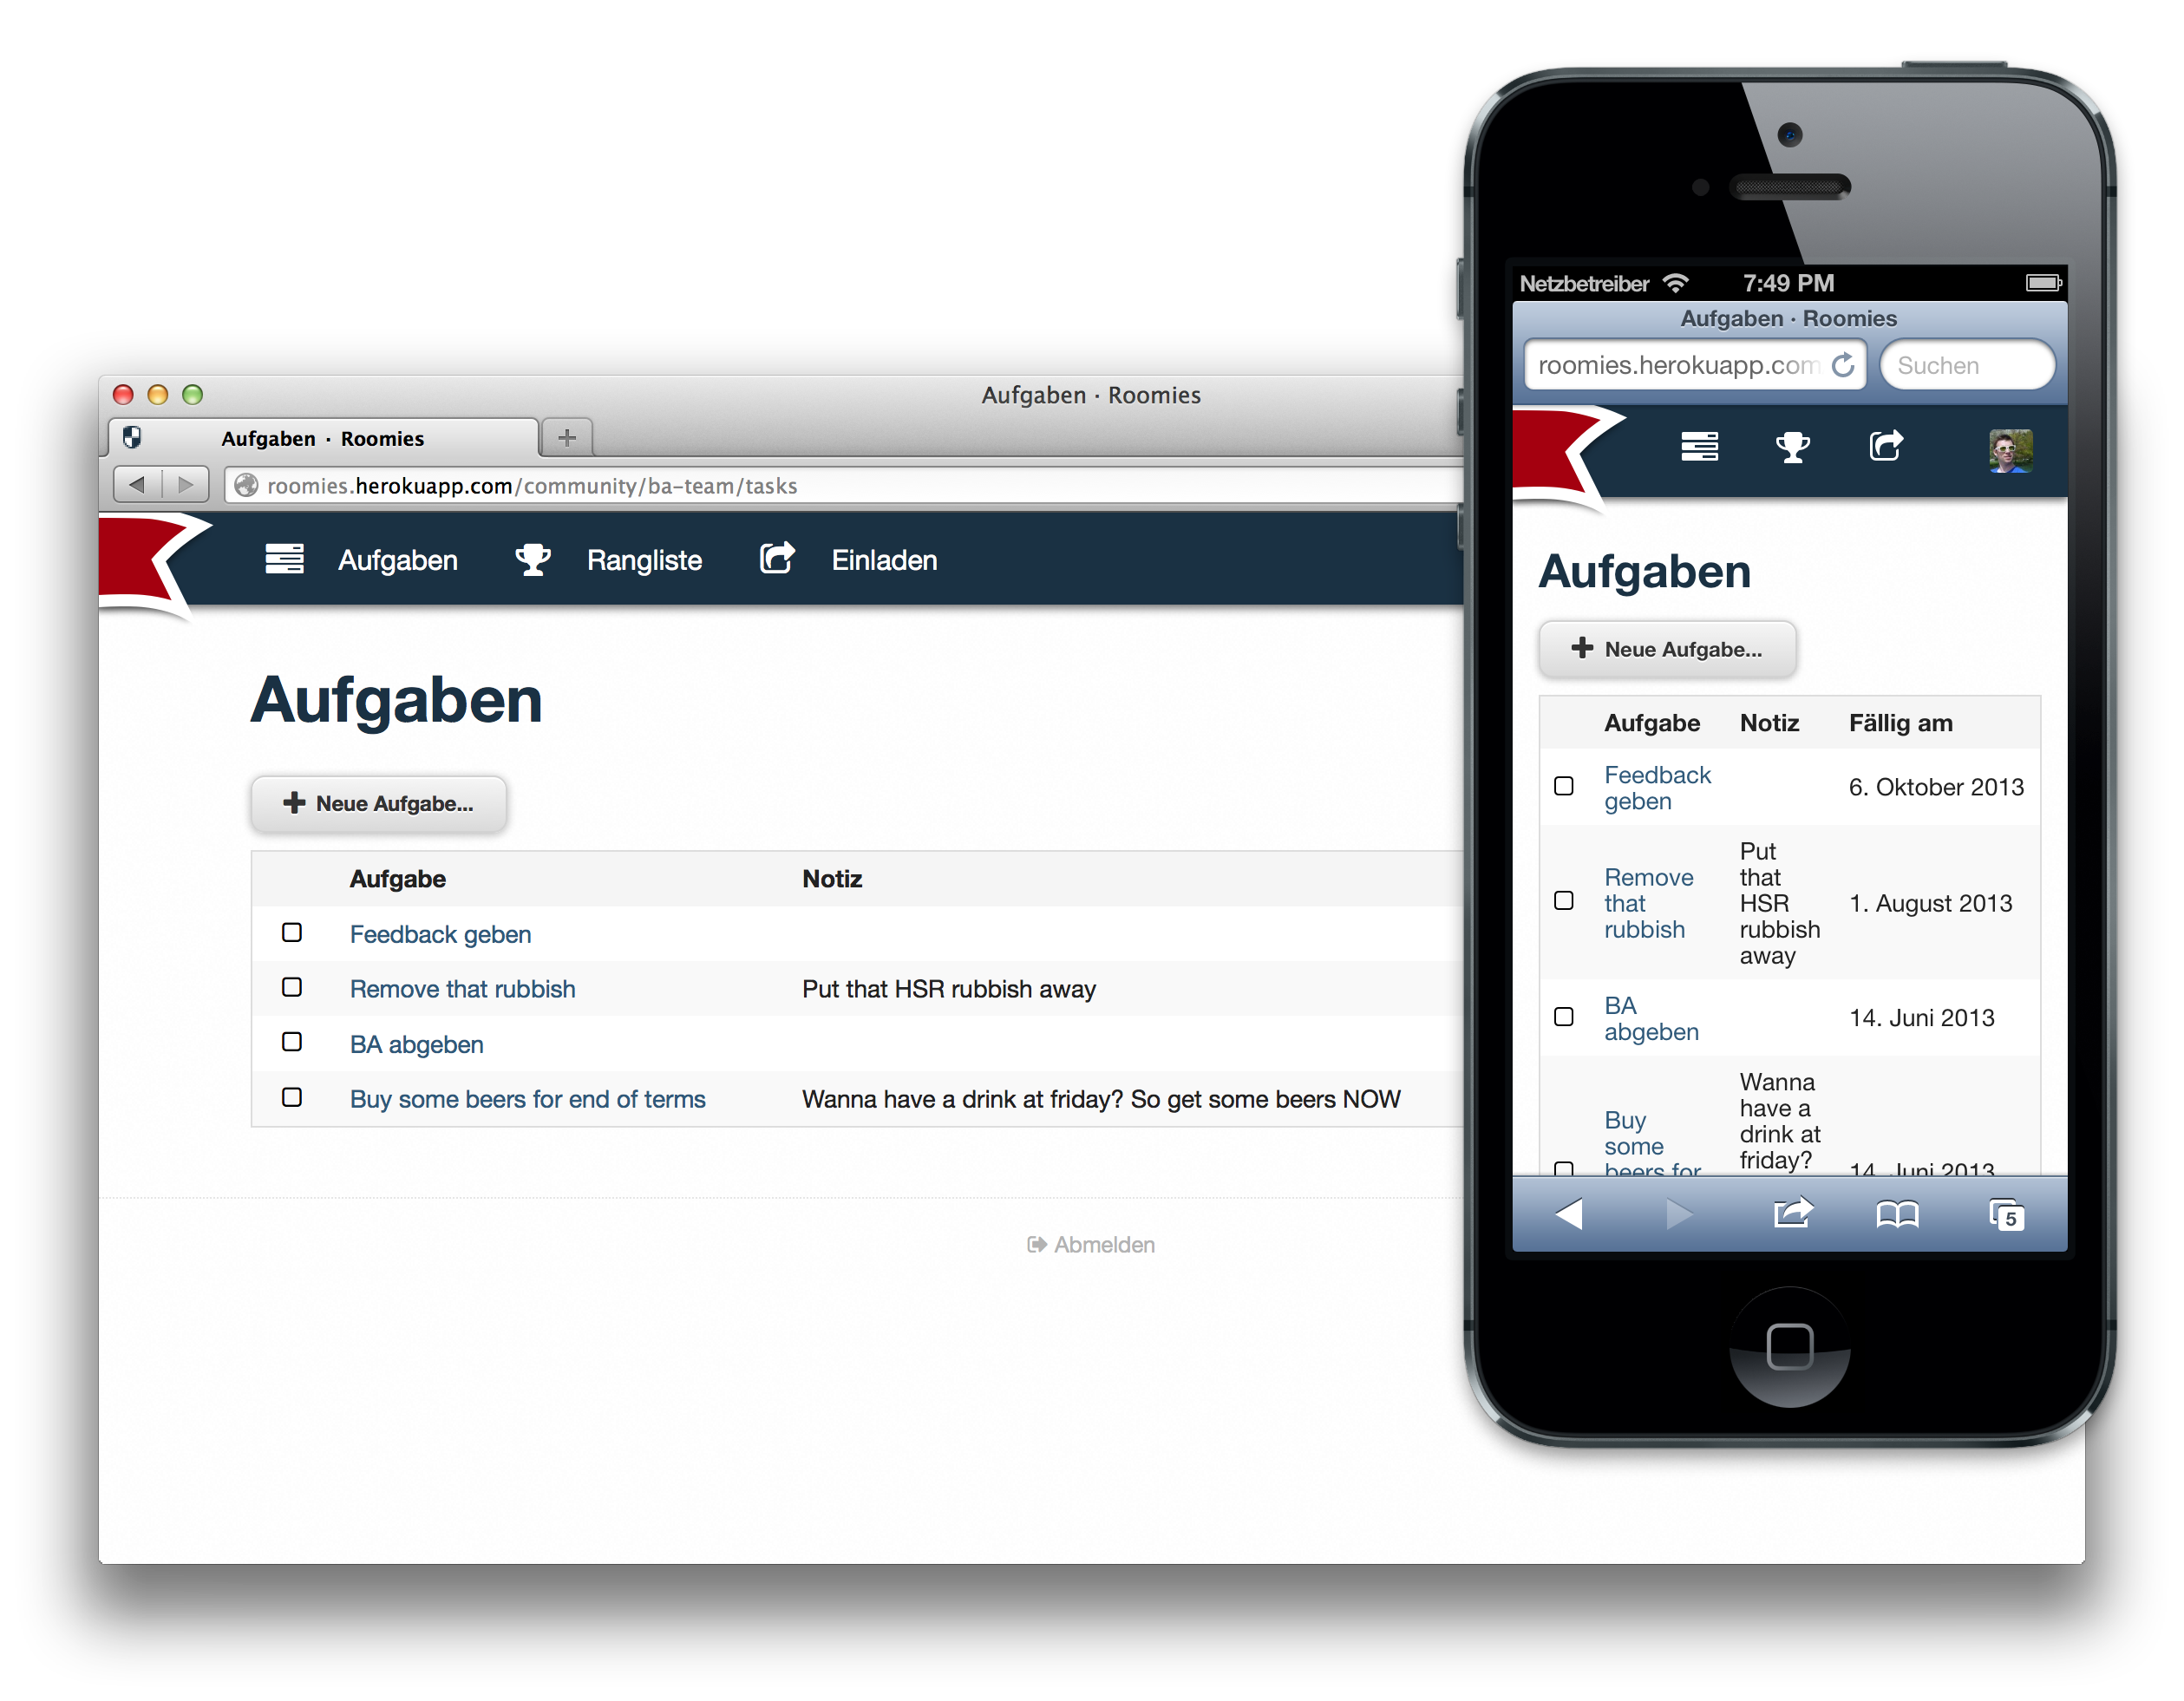
\includegraphics[width=12cm]{content/principle-demonstration/images/responsive-screenshots.png}
	\caption{Aufgabenverwaltung \emph{Roomies} zur Konzeptdemonstration}
\end{figure}

Währen den ersten Arbeiten an der Beispielapplikation wurde dem Projektteam schnell klar, dass die Anforderungen der \emph{Unobtrusive JavaScript}-Richtlinie einiges mehr an Aufwand verschlingen würden als zuerst angenommen wurde. Die Anstrengungen in diesem Gebiet wurden mit dem wiederverwendbaren Framework \emph{barefoot} belohnt: Unter dessen Integration kann \emph{Roomies}' Quellcode ohne mehrfache Implementation sowohl auf dem Server als auch auf dem Client verwendet werden.






Die Studie am Ende dieser Bachelorarbeit bietet einen tiefen Einblick in die Entwicklung einer verteilten, JavaScript-basierten Client-Server-Webapplikation. Die ausführlichen Analysen und persönlichen Stellungnahmen des gesamten Projektteams bewerten die untersuchten Softwarearchitekturkonzepte kritisch. Ergänzend dazu bietet der Quellcode von ``Roomies'' anschauliche Beispiele zu jedem der 22 Konzepte. Besondere Aufmerksamkeit wurde dabei dem Konzept ``Unobtrusive JavaScript'' zuteil. Basierend auf ``Backbone.js'' wurde eine eigene quelloffene Bibliothek namens ``barefoot'' entwickelt, welche ohne grösseren Mehraufwand den gleichen Quelltext sowohl im Browser des Endbenutzers als auch auf der Serverkomponente lauffähig macht.


\section{Ausblick}

Der vorliegenden Bericht hat mit seinen ausführlichen Analysen vorgestellter Richtlinien eine umfassende Grundlage zur Konzipierung neuer Inhalte im Unterrichtsmodul \emph{Internettechnologien} geschaffen. Zusammen mit der Beispielapplikation bildet er ein Gesamtpaket aus theoretischen und praktischen Beispielen. Das Projektteam hofft, mit diesen Ergebnisse einen grossen Beitrag zur Weiterentwicklung der Vorlesung und den Übungslektionen leisten zu können.

Als drittes, offizielles Produkt wurde mit \emph{barefoot} eine frei zugängliche Bibliothek veröffentlicht. Das Projektteam ist davon überzeugt, dass diese für andere Projekte von grossem Nutzen ist. Um das Fortbestehen der Bibliothek zu sichern, hat sich das Projektteam darum entschieden, nach Abschluss dieser Bachelorarbeit für den Unterhalt und die Weiterentwicklung von \emph{barefoot} zu sorgen.

















\chapter{Schlussfolgerung}

\section*{Roll Up}

In den vorangegangenen drei Kapiteln hat sich das Projektteam ausführlich mit den verschiedenen Aspekten moderner Webapplikationen befasst. Es wurde eine Zusammenstellung von Architekturrichtlinien analysiert und dabei jedes Konzept aus unterschiedlichen Perspektiven sowohl theoretisch als auch praktisch bewertet.

Nach der Evaluation dreier Technologiekandidaten und mehrerer Bibliotheken wurde unter Verwendung von \emph{JavaScript} und \emph{Express.js} mit \emph{Roomies} eine Applikation zur Veranschaulichung der ausgewählten Konzepte entwickelt.

Währen den ersten Arbeiten an der Beispielapplikation wurde dem Projektteam schnell klar, dass die Anforderungen der \emph{Unobtrusive JavaScript}-Richtlinie einiges mehr an Aufwand verschlingen würden als zuerst angenommen wurde. Die Anstrengungen in diesem Gebiet wurden mit dem wiederverwendbaren Framework \emph{barefoot} belohnt: Unter dessen Integration kann \emph{Roomies}' Quellcode ohne mehrfache Implementation sowohl auf dem Server als auch auf dem Client verwendet werden.


\section*{Fazit}


\subsection*{Architekturrichtlinien}

Aus über 25 Richtlinien, Architekturkonzepten und Prinzipien wurden während der Vorselektion insgesamt 22 ausgewählt, um in einem weiteren Schritt am praktischen Beispiel \emph{Roomies} demonstriert zu werden.

Bis auf einige wenige Ausnahmen konnten alle Konzepte befriedigend implementiert werden. Dabei stechen \emph{No Duplication} und \emph{Unobtrusive JavaScript} aus dem ROCA-Katalog besonders hervor:

Während der Implementation von \emph{Roomies} flossen über 40 Prozent des Gesamtaufwandes in die Umsetzung dieser Richtlinien. Insbesondere die Integration bestehender Codefragmente mit \emph{barefoot} verschlang ausserordentlich viel Zeit.

Die Qualität von \emph{barefoot} konnte von diesem Prozess hingegen sehr profitieren. In dessen aktueller Version \emph{0.0.11} sind viele der ursprünglichen Fehler behoben und wichtige Features wurden ergänzt oder neu konzipiert.

Negativ aufgefallen sind lediglich die Konzepte \emph{Know Structure} und \emph{Auth}: Ersteres war mit der Umsetzung von \emph{Unobtrusive JavaScript} nicht zu vereinbaren, da diese miteinander im Widerspruch stehen. \emph{Auth} wurde gezielt nicht umgesetzt, um den Workload auf das Team zu optimieren.

Gesamtheitlich schätzt das Projektteam die bearbeiteten Architekturrichtlinien als zweckmässig und sehr hilfreich ein. Vielerorts muss jedoch wie dokumentiert von Situation zu Situation entschieden werden, welchen Konzepten aufgrund der vorliegenden Anforderungen der Vorzug gewährt wird.


\subsection*{Tauglichkeit das für Unterrichtsmodul Internettechnologien}

Seit der gemeinsamen Definition der Aufgabenstellung gehörte die Idee, neue Vorschläge für das Unterrichtmodul \emph{Internettechnologien} zu liefern, fest zum Thema dieser Bachelorarbeit dazu.

Neben der praktischen Demonstration sollte insbesondere auch der theoretische Teil der Arbeit darüber Aufschluss geben, inwiefern die neuen, zu untersuchenden Architekturkonzepte für den Unterricht und damit den Entwickleralltag tauglich sind.

Mit der Beispielapplikation \emph{Roomies} sind alle Richtlinien bis auf zwei Ausnahmen praktisch umgesetzt und demonstriert worden. Das vorliegende Produkt verfügt über eine klare und durchgehende Komponentenarchitektur. Das Projektteam ist davon überzeugt, dass Aspekte wie die \emph{REST}-basierte API oder das umgesetzte \emph{MVC}-Pattern für das User Interface Mustergültigkeit haben.

Im grösseren Zusammenspiel, insbesondere in Kombination mit dem \emph{Express.js Middleware}-Konzept sowie dem experimentellen \emph{Code Sharing}-Ansatz \emph{barefoot}s, ergibt sich eine komplexe Kombination der für sich einfachen Komponenten. Das Projektteam ist sich deshalb nicht sicher, in wie weit die Beispielapplikation als Ganzes tatsächlich in den Unterricht integriert werden kann.

Die vollständige Analyse der Richtlinien im Kapitel \ref{sec:principle-demonstration} ``\nameref{sec:principle-demonstration}'' bietet eine optimale Grundlage für das Übertragen der untersuchten Prinzipien in den Unterricht. Ausführliche Quellenangaben und Querverweise erleichtern zudem das Erarbeiten weiterführender Themen. So hält das Projektteam diesen Teil des Arbeitsergebnisses für uneingeschränkt wertvoll und wiederverwendbar.


\subsection*{Kontroverse: JavaScript}

Während der Technologieevaluation war umstritten, ob \emph{JavaScript} wirklich für den geplanten Einsatz vollumfänglich geeignet sei. Zwar wurden bereits Lösungen mit \emph{Node.js} für den produktiven Einsatz umgesetzt und auch das Projektteam hat in der Studienarbeit positive Erfahrung auf der Clientseite machen können. Trotzdem waren altbekannte Unsicherheiten teils weiterhin sowohl im Betreuer- als auch Projektteam spürbar:

\begin{itemize}
	\item Seriöses Software Engineering (\emph{Separation Of Concerns}, \gls{TDD}, CI etc.) ist mit \emph{JavaScript} nicht möglich
	\item Schlechte serverseitige Performance
	\item Schlechte Strukturierung von Quellcode (\emph{Callback Hell} etc.)
\end{itemize}

Die gemachten Erfahrungen mit der Umsetzung von \emph{Roomies} beweisen, dass \emph{JavaScript} sich sehr wohl mit bekannten Technologien wie \emph{Ruby} messen kann. Gerade in den Belangen Flexibilität und Skalierbarkeit braucht es sich keinesfalls zu verstecken.

Werkzeuge wie \emph{JSHint}, \emph{Mocha}, \emph{Travis CI} oder \emph{JSCoverage} ermöglichen die Sicherstellung der Codequalität von \emph{JavaScript} Quelltext-Artefakten.

\emph{JavaScript} ist definitiv seinen Kinderschuhen entwachsen und wird rege weiterentwickelt. Das Projektteam hat die Entscheidung für \emph{JavaScript} keine Sekunde bereut und kann auch nach erfolgreicher Durchführung dieser Arbeit voll und ganz hinter dieser Entscheidung stehen.


\section*{Ausblick}


